\chapter{Numbers and Base-3 Arithmetic}
\label{ch:numbers}

\begin{chapterobjectives}
\textbf{Prerequisites:} None. This chapter starts from the very beginning.

\textbf{What you'll learn:}
\begin{itemize}
\item 🟢 How to count in different bases (especially base-3)
\item 🟡 The digital sum function $D_3(n)$ and its properties
\item 🔴 Connection to fractal patterns and number theory
\end{itemize}

\textbf{Why this matters:} The base-3 digital sum function is the foundation of the fractal resonance function $R_f(\alpha, s)$, which appears throughout this entire framework. Understanding how base-3 works is essential for everything that follows.
\end{chapterobjectives}

\section{Counting Systems Throughout History}
\label{sec:counting-systems}

\subsection{How We Count: It's Not as Simple as You Think}
\label{subsec:intuitive-bases}

% ============================================================
% LEVEL 1: INTUITIVE (🟢) - For everyone
% ============================================================

When you see the number "27", what does it mean?

This seems like a silly question, but the answer reveals something profound: \textit{the way we write numbers is just a convention}. Throughout history, humans have invented many different ways to represent the same quantity.

\begin{intuitive}[title=Why Do We Use Ten Fingers?]
Most of us learned to count in \textbf{base-10} (also called "decimal"). When you write "27", you mean:
\begin{equation}
27 = 2 \times 10 + 7 \times 1
\end{equation}

But why 10? Because humans typically have 10 fingers! This is literally where our counting system comes from. It's not mathematically special—it's just convenient for creatures with ten digits.
\end{intuitive}

\subsubsection*{A Journey Through Counting Systems}

Let's see how different civilizations tackled this problem:

\paragraph{The Babylonians (3000 BCE):} Used \textbf{base-60}. Why? Nobody knows for certain, but 60 has many divisors (1, 2, 3, 4, 5, 6, 10, 12, 15, 20, 30, 60), making it convenient for fractions. We still use base-60 today for time (60 seconds, 60 minutes) and angles (360° = 6×60).

\textit{Example:} The number we call "90" would be written as "1,30" in Babylonian (meaning 1×60 + 30).

\paragraph{The Romans (500 BCE - 500 CE):} Used letters as numbers:
\begin{center}
I=1, \quad V=5, \quad X=10, \quad L=50, \quad C=100, \quad D=500, \quad M=1000
\end{center}

This system works, but try multiplying XXVII by XIV in your head. (That's 27 × 14 = 378 = CCCLXXVIII. Not fun!)

\paragraph{Hindu-Arabic System (500 CE):} The system we use today, with the revolutionary invention of \textbf{zero} as a placeholder. This made arithmetic dramatically easier.

\paragraph{Binary - Base-2 (1700s):} Gottfried Leibniz explored base-2, using only digits \{0, 1\}. Every number is powers of 2. In the 1940s, this became the foundation of all digital computers.

\textit{Example:} The number "27" in binary is "11011":
\begin{equation}
11011_2 = 1×16 + 1×8 + 0×4 + 1×2 + 1×1 = 27
\end{equation}

\paragraph{Ternary - Base-3 (This Framework):} Uses only digits \{0, 1, 2\}\index{base-3}\index{ternary}. Every number is powers of 3. This is what we'll focus on.

\textit{Example:} The number "27" in base-3 is "1000":
\begin{equation}
1000_3 = 1×27 + 0×9 + 0×3 + 0×1 = 27
\end{equation}

\begin{intuitive}[title=Understanding Any Base]
In base-$b$, you use digits from 0 to $b-1$, and positions represent powers of $b$:

\begin{center}
\begin{tabular}{ccccc}
... & $b^3$ place & $b^2$ place & $b^1$ place & $b^0$ place \\
\hline
& thousands & hundreds & tens & ones \\
\end{tabular}
\end{center}

\textbf{Base-10:} digits \{0,1,2,3,4,5,6,7,8,9\}, positions are powers of 10

\textbf{Base-3:} digits \{0,1,2\}, positions are powers of 3

\textbf{Base-2:} digits \{0,1\}, positions are powers of 2
\end{intuitive}

\begin{figure}[h]
\centering
% Figure 1.1: Timeline of Number Systems
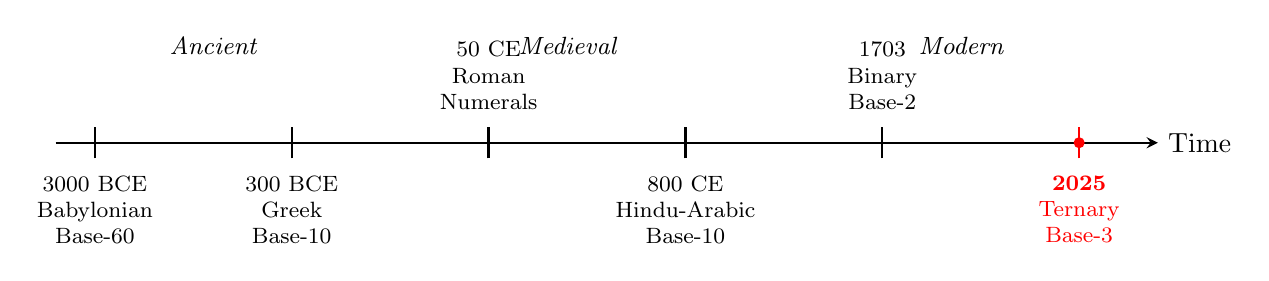
\begin{tikzpicture}[scale=1.0]
  % Timeline axis
  \draw[thick, ->, >=stealth] (0,0) -- (14,0) node[right] {Time};

  % Historical markers
  \def\timelinedata{
    {0.5, "3000 BCE", "Babylonian", "Base-60"},
    {3.0, "300 BCE", "Greek", "Base-10"},
    {5.5, "50 CE", "Roman", "Numerals"},
    {8.0, "800 CE", "Hindu-Arabic", "Base-10"},
    {10.5, "1703", "Binary", "Base-2 (Leibniz)"},
    {13.0, "2025", "Ternary", "Base-3 (This Book)"}
  }

  % Babylonian (3000 BCE)
  \draw[thick] (0.5,-0.2) -- (0.5,0.2);
  \node[below, align=center, font=\footnotesize] at (0.5,-0.3) {3000 BCE\\Babylonian\\Base-60};

  % Greek (300 BCE)
  \draw[thick] (3.0,-0.2) -- (3.0,0.2);
  \node[below, align=center, font=\footnotesize] at (3.0,-0.3) {300 BCE\\Greek\\Base-10};

  % Roman (50 CE)
  \draw[thick] (5.5,-0.2) -- (5.5,0.2);
  \node[above, align=center, font=\footnotesize] at (5.5,0.3) {50 CE\\Roman\\Numerals};

  % Hindu-Arabic (800 CE)
  \draw[thick] (8.0,-0.2) -- (8.0,0.2);
  \node[below, align=center, font=\footnotesize] at (8.0,-0.3) {800 CE\\Hindu-Arabic\\Base-10};

  % Binary (1703)
  \draw[thick] (10.5,-0.2) -- (10.5,0.2);
  \node[above, align=center, font=\footnotesize] at (10.5,0.3) {1703\\Binary\\Base-2};

  % Ternary (2025) - highlighted
  \draw[thick, red] (13.0,-0.2) -- (13.0,0.2);
  \node[below, align=center, font=\footnotesize, red] at (13.0,-0.3) {\textbf{2025}\\Ternary\\Base-3};
  \fill[red] (13.0,0) circle (2pt);

  % Era labels
  \node[above, font=\small\itshape] at (2.0,1.0) {Ancient};
  \node[above, font=\small\itshape] at (6.5,1.0) {Medieval};
  \node[above, font=\small\itshape] at (11.5,1.0) {Modern};

\end{tikzpicture}

\caption{Timeline of number systems throughout history. Base-3 (ternary) represents the most recent addition to our mathematical toolkit, building on millennia of human innovation in representing quantities.}
\label{fig:timeline}
\end{figure}

\subsubsection*{Why Base-3 Is Special for This Framework}

You might wonder: "If base-10 is convenient for humans and base-2 is convenient for computers, why do we care about base-3?"

The answer will become clear throughout this book, but here's a preview:

\begin{keyidea}[title=The Magic of Three]
Base-3 is not arbitrary—it appears throughout nature and human biology:
\begin{itemize}
\item \textbf{Human Anatomy:} Each of our 4 fingers has 3 phalanges (bone segments). Our ancestors counted by using the thumb to point at each phalange segment: 1, 2, 3 on the index finger, then 4, 5, 6 on the middle finger, and so on. This gives us natural base-3 counting up to 12 on one hand (4 fingers × 3 segments). While base-10 counts fingers, base-3 counts the \textit{segments within} fingers.
\item \textbf{Physics:} Quantum systems often have three-way symmetries (particle triality, three generations of matter, three color charges in quarks)
\item \textbf{Mathematics:} Many deep structures have mod-3 properties (cubic reciprocity, ternary expansions)
\item \textbf{Computation:} Ternary logic can be more efficient than binary (balanced ternary uses \{-1, 0, +1\})
\item \textbf{This Framework:} The digital sum of base-3 representations creates fractal patterns that unlock solutions to fundamental problems
\end{itemize}
\end{keyidea}

\begin{figure}[h]
\centering
% Figure 1.2: Number 27 in Different Bases
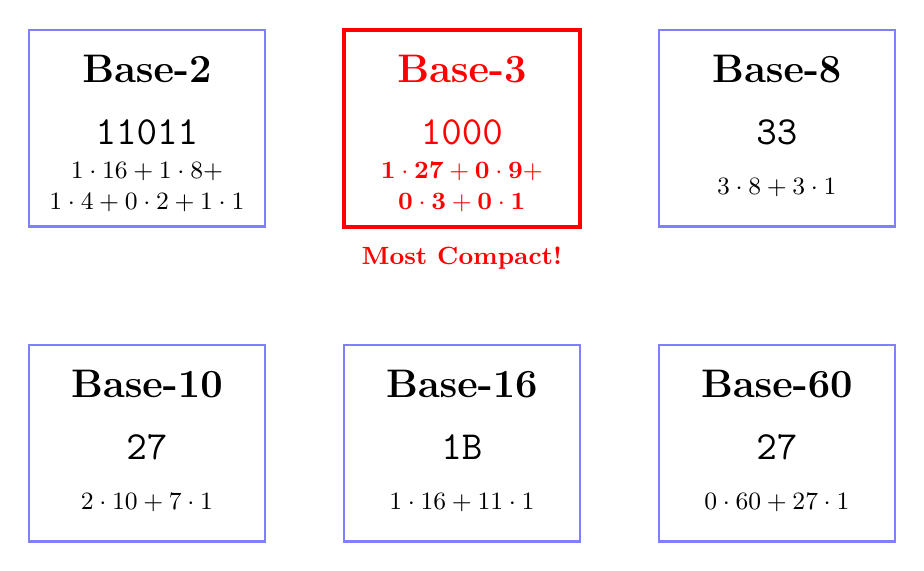
\begin{tikzpicture}[scale=1.0]

  % Title (implicit - will be in caption)

  % Base-2 (Binary)
  \node[font=\Large\bfseries] at (0,5) {Base-2};
  \node[font=\ttfamily\Large] at (0,4.2) {11011};
  \node[font=\small, align=center] at (0,3.5) {$1 \cdot 16 + 1 \cdot 8 +$\\$1 \cdot 4 + 0 \cdot 2 + 1 \cdot 1$};
  \draw[thick, draw=blue!50] (-1.5,3.0) rectangle (1.5,5.5);

  % Base-3 (Ternary) - highlighted
  \node[font=\Large\bfseries, red] at (4,5) {Base-3};
  \node[font=\ttfamily\Large, red] at (4,4.2) {1000};
  \node[font=\small, align=center, red] at (4,3.5) {$\mathbf{1 \cdot 27 + 0 \cdot 9 +}$\\$\mathbf{0 \cdot 3 + 0 \cdot 1}$};
  \draw[thick, draw=red, line width=1.5pt] (2.5,3.0) rectangle (5.5,5.5);
  \node[font=\small, red] at (4,2.6) {\textbf{Most Compact!}};

  % Base-8 (Octal)
  \node[font=\Large\bfseries] at (8,5) {Base-8};
  \node[font=\ttfamily\Large] at (8,4.2) {33};
  \node[font=\small, align=center] at (8,3.5) {$3 \cdot 8 + 3 \cdot 1$};
  \draw[thick, draw=blue!50] (6.5,3.0) rectangle (9.5,5.5);

  % Base-10 (Decimal)
  \node[font=\Large\bfseries] at (0,1.0) {Base-10};
  \node[font=\ttfamily\Large] at (0,0.2) {27};
  \node[font=\small, align=center] at (0,-0.5) {$2 \cdot 10 + 7 \cdot 1$};
  \draw[thick, draw=blue!50] (-1.5,-1.0) rectangle (1.5,1.5);

  % Base-16 (Hexadecimal)
  \node[font=\Large\bfseries] at (4,1.0) {Base-16};
  \node[font=\ttfamily\Large] at (4,0.2) {1B};
  \node[font=\small, align=center] at (4,-0.5) {$1 \cdot 16 + 11 \cdot 1$};
  \draw[thick, draw=blue!50] (2.5,-1.0) rectangle (5.5,1.5);

  % Base-60 (Babylonian)
  \node[font=\Large\bfseries] at (8,1.0) {Base-60};
  \node[font=\ttfamily\Large] at (8,0.2) {27};
  \node[font=\small, align=center] at (8,-0.5) {$0 \cdot 60 + 27 \cdot 1$};
  \draw[thick, draw=blue!50] (6.5,-1.0) rectangle (9.5,1.5);

\end{tikzpicture}

\caption{The number 27 represented in different bases. Notice how base-3 (ternary) gives the most compact representation: just "1000". This compactness is one reason why base-3 is mathematically elegant.}
\label{fig:bases}
\end{figure}

\subsubsection*{Converting Between Bases: A Simple Recipe}

Let's learn how to convert any number to base-3. We'll use 27 as our example.

\begin{example}[title=Converting 27 to Base-3]
\textbf{Method:} Repeatedly divide by 3 and track remainders:

\begin{align}
27 ÷ 3 &= 9 \text{ remainder } \boxed{0} \\
9 ÷ 3 &= 3 \text{ remainder } \boxed{0} \\
3 ÷ 3 &= 1 \text{ remainder } \boxed{0} \\
1 ÷ 3 &= 0 \text{ remainder } \boxed{1}
\end{align}

Read the remainders \textit{bottom to top}: $\boxed{1}\boxed{0}\boxed{0}\boxed{0}$

Therefore: $27_{10} = 1000_3$ \checkmark

\textbf{Verification:}
\begin{equation}
1×3^3 + 0×3^2 + 0×3^1 + 0×3^0 = 1×27 + 0 + 0 + 0 = 27 \checkmark
\end{equation}
\end{example}

\begin{tryit}[title=Your Turn]
Convert these numbers to base-3 using the method above:
\begin{enumerate}
\item $n = 5$ (Answer: $12_3$)
\item $n = 10$ (Answer: $101_3$)
\item $n = 20$ (Answer: $202_3$)
\end{enumerate}

Detailed solutions are in Appendix F, Section F.1.
\end{tryit}

\subsubsection*{The Digital Sum: Adding Digits Together}

Now comes the key concept for this entire framework: the \textbf{digital sum}.

\begin{definition}[title=Digital Sum in Base-3]
For any positive integer $n$, write it in base-3. The \textbf{digital sum}\index{digital sum}\index{D3@$D_3(n)$} $D_3(n)$ is simply the sum of its base-3 digits.
\end{definition}

\begin{example}[title=Computing $D_3(27)$]
Step 1: Convert to base-3: $27 = 1000_3$

Step 2: Add the digits: $D_3(27) = 1 + 0 + 0 + 0 = 1$

That's it! $D_3(27) = 1$.
\end{example}

\begin{example}[title=Computing $D_3(10)$]
Step 1: Convert to base-3: $10 = 101_3$

Step 2: Add the digits: $D_3(10) = 1 + 0 + 1 = 2$

Therefore $D_3(10) = 2$.
\end{example}

Let's compute $D_3(n)$ for the first few numbers:

\begin{center}
\begin{tabular}{c|c|c|c}
$n$ & Base-10 & Base-3 & $D_3(n)$ \\
\hline
1 & 1 & 1 & 1 \\
2 & 2 & 2 & 2 \\
3 & 3 & 10 & 1 \\
4 & 4 & 11 & 2 \\
5 & 5 & 12 & 3 \\
6 & 6 & 20 & 2 \\
7 & 7 & 21 & 3 \\
8 & 8 & 22 & 4 \\
9 & 9 & 100 & 1 \\
10 & 10 & 101 & 2 \\
\end{tabular}
\end{center}

\begin{intuitive}[title=What Do You Notice?]
Look at the pattern in the $D_3(n)$ column: 1, 2, 1, 2, 3, 2, 3, 4, 1, 2, ...

\begin{itemize}
\item It's not just increasing
\item It has a repeating structure
\item It "resets" at powers of 3 (at $n=3$: $D_3(3)=1$, at $n=9$: $D_3(9)=1$)
\end{itemize}

This is a \textbf{fractal pattern}\index{fractal!pattern}—it repeats at different scales. This self-similarity\index{self-similarity} is the key to everything in this book.
\end{intuitive}

\begin{historicalnote}[title=Leibniz and Binary]
Gottfried Wilhelm Leibniz (1646-1716) was fascinated by binary (base-2) for philosophical reasons. He saw parallels with creation (1) and nothingness (0), and with Chinese philosophy (Yang and Yin). In his 1703 paper \textit{Explication de l'Arithmétique Binaire}, he wrote:

\begin{quote}
\textit{"The binary system is the simplest of all, using only 0 and 1... It demonstrates that everything can be created from nothing through the power of unity."}
\end{quote}

Three centuries later, this became the foundation of digital computing. Now, we explore what base-3 reveals about the structure of mathematics itself.
\end{historicalnote}

\subsection{Summary of Section 1.1}

\textbf{Key Points:}
\begin{enumerate}
\item Number bases are conventions—base-10 is not special, just convenient for humans
\item Different civilizations used different bases (Babylonian 60, Roman letters, Hindu-Arabic 10, Binary 2)
\item Base-3 uses only digits \{0, 1, 2\} with positions as powers of 3
\item The digital sum $D_3(n)$ = sum of base-3 digits of $n$
\item $D_3(n)$ exhibits fractal patterns that will be central to this framework
\end{enumerate}

\textbf{Next:} In Section 1.2, we'll explore the beautiful fractal patterns in $D_3(n)$ more deeply and prove why these patterns exist.

% End of Section 1.1

\section{Patterns in Digital Sums}
\label{sec:digital-sum-patterns}

Now that we understand how to compute $D_3(n)$, let's explore the beautiful patterns hidden in this simple function. What appears at first to be just "adding digits" reveals itself to be a fractal structure with deep mathematical significance.

\subsection{Visualizing the Pattern}
\label{subsec:visualizing-pattern}

% ============================================================
% LEVEL 1: INTUITIVE (🟢) - Visual exploration
% ============================================================

Let's compute $D_3(n)$ for the first 27 numbers and see what emerges:

\begin{center}
\begin{tabular}{c|c|c||c|c|c||c|c|c}
$n$ & Base-3 & $D_3(n)$ & $n$ & Base-3 & $D_3(n)$ & $n$ & Base-3 & $D_3(n)$ \\
\hline
1 & 1 & 1 & 10 & 101 & 2 & 19 & 201 & 3 \\
2 & 2 & 2 & 11 & 102 & 3 & 20 & 202 & 4 \\
3 & 10 & 1 & 12 & 110 & 2 & 21 & 210 & 3 \\
4 & 11 & 2 & 13 & 111 & 3 & 22 & 211 & 4 \\
5 & 12 & 3 & 14 & 112 & 4 & 23 & 212 & 5 \\
6 & 20 & 2 & 15 & 120 & 3 & 24 & 220 & 4 \\
7 & 21 & 3 & 16 & 121 & 4 & 25 & 221 & 5 \\
8 & 22 & 4 & 17 & 122 & 5 & 26 & 222 & 6 \\
9 & 100 & 1 & 18 & 200 & 2 & 27 & 1000 & 1 \\
\end{tabular}
\end{center}

\begin{intuitive}[title=What Do You See?]
Look at the $D_3(n)$ column carefully:

\textbf{From 1-9:} 1, 2, 1, 2, 3, 2, 3, 4, 1

\textbf{From 10-18:} 2, 3, 2, 3, 4, 3, 4, 5, 2

\textbf{From 19-27:} 3, 4, 3, 4, 5, 4, 5, 6, 1

Notice three things:
\begin{enumerate}
\item The pattern has a basic "shape" that repeats
\item Each repetition is shifted up by 1
\item At powers of 3 ($n = 3, 9, 27$), we get $D_3(n) = 1$ (a "reset")
\end{enumerate}

This is \textbf{self-similarity}—the hallmark of fractals!
\end{intuitive}

\subsubsection*{The Fractal Staircase}

If we plot $D_3(n)$ versus $n$, we get what looks like a staircase with repeating sub-structures:

\begin{figure}[h]
\centering
% Figure 1.3: D₃(n) Pattern for n = 1 to 27
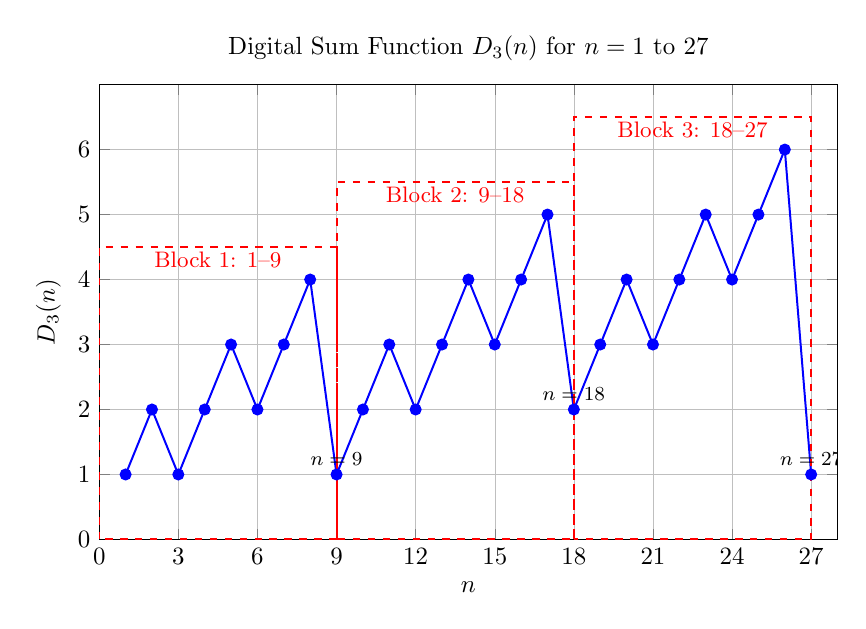
\begin{tikzpicture}[scale=0.9]
\begin{axis}[
    width=12cm,
    height=8cm,
    xlabel={$n$},
    ylabel={$D_3(n)$},
    title={Digital Sum Function $D_3(n)$ for $n = 1$ to $27$},
    xmin=0, xmax=28,
    ymin=0, ymax=7,
    xtick={0,3,6,9,12,15,18,21,24,27},
    ytick={0,1,2,3,4,5,6},
    grid=both,
    grid style={line width=.1pt, draw=gray!10},
    major grid style={line width=.2pt,draw=gray!50},
    legend pos=north west,
]

% Data points for D₃(n)
% n=1: 1, n=2: 2, n=3: 1, n=4: 1+1=2, n=5: 1+2=3, n=6: 2+0=2, n=7: 2+1=3, n=8: 2+2=4, n=9: 1
% n=10: 1+0+1=2, n=11: 1+0+2=3, n=12: 1+1+0=2, n=13: 1+1+1=3, etc.

\addplot[
    color=blue,
    mark=*,
    mark size=2pt,
    thick
] coordinates {
(1,1) (2,2) (3,1) (4,2) (5,3) (6,2) (7,3) (8,4) (9,1)
(10,2) (11,3) (12,2) (13,3) (14,4) (15,3) (16,4) (17,5) (18,2)
(19,3) (20,4) (21,3) (22,4) (23,5) (24,4) (25,5) (26,6) (27,1)
};

% Highlight the repeating pattern blocks
\draw[red, thick, dashed] (axis cs:0,0) rectangle (axis cs:9,4.5);
\node[red, font=\small] at (axis cs:4.5,4.3) {Block 1: 1--9};

\draw[red, thick, dashed] (axis cs:9,0) rectangle (axis cs:18,5.5);
\node[red, font=\small] at (axis cs:13.5,5.3) {Block 2: 9--18};

\draw[red, thick, dashed] (axis cs:18,0) rectangle (axis cs:27,6.5);
\node[red, font=\small] at (axis cs:22.5,6.3) {Block 3: 18--27};

% Annotate special points
\node[above, font=\footnotesize] at (axis cs:9,1) {$n=9$};
\node[above, font=\footnotesize] at (axis cs:18,2) {$n=18$};
\node[above, font=\footnotesize] at (axis cs:27,1) {$n=27$};

\end{axis}
\end{tikzpicture}

\caption{The digital sum function $D_3(n)$ for $n = 1$ to $27$. Notice the three self-similar blocks: 1--9, 9--18, and 18--27. Each block repeats the same pattern, shifted upward by 1, and resets at powers of 3 ($n = 9, 18, 27$).}
\label{fig:d3pattern}
\end{figure}

The pattern repeats at three scales:
\begin{itemize}
\item \textbf{Scale 1 (fine):} Within each group of 3 numbers
\item \textbf{Scale 2 (medium):} Within each group of 9 numbers  
\item \textbf{Scale 3 (coarse):} Within each group of 27 numbers
\end{itemize}

And this continues forever! Groups of 81, groups of 243, groups of 729...

\begin{keyidea}[title=Fractal Self-Similarity]
A fractal is a pattern that looks similar at different scales. The famous Mandelbrot set, coastlines, and branching trees all exhibit this property.

The $D_3(n)$ function is fractal because:
$$D_3(3k + r) = D_3(k) + D_3(r)$$

This means the pattern at position $n$ depends on the pattern at position $n/3$, which depends on the pattern at position $n/9$, and so on—creating recursive structure at all scales.
\end{keyidea}

\subsection{Computational Exploration}
\label{subsec:computational-exploration}

Let's write code to explore these patterns systematically.

\begin{lstlisting}[language=Python, caption=Computing $D_3(n)$ efficiently]
def D3(n):
    """Compute base-3 digital sum of n"""
    digit_sum = 0
    while n > 0:
        digit_sum += n % 3
        n //= 3
    return digit_sum

# Compute for first 100 numbers
values = [D3(n) for n in range(1, 101)]

# Find pattern properties
print(f"Maximum value in first 100: {max(values)}")
print(f"Minimum value in first 100: {min(values)}")

# Check for periodicity
def find_period(sequence, max_period=50):
    n = len(sequence)
    for p in range(1, min(max_period, n//2)):
        if sequence[:p] == sequence[p:2*p]:
            return p
    return None

period = find_period(values)
print(f"Period (if exists): {period}")
\end{lstlisting}

\begin{example}[title=Running the Code]
When you run this code, you'll find:
\begin{itemize}
\item Maximum value grows logarithmically (roughly $\log_3(n)$)
\item Minimum value is always 1 (at powers of 3)
\item There's no simple period—the pattern is fractal, not periodic
\end{itemize}
\end{example}

% ============================================================
% LEVEL 2: TECHNICAL (🟡) - Formal mathematics
% ============================================================

\subsection{Mathematical Properties}
\label{subsec:mathematical-properties}

Now let's prove rigorously why these patterns exist.

\begin{definition}[title=Digital Sum Function]
For $n \in \mathbb{N}$, let $n = \sum_{k=0}^{m} d_k \cdot 3^k$ be the base-3 representation with $d_k \in \{0,1,2\}$. The \textbf{digital sum} is:
$$D_3(n) := \sum_{k=0}^{m} d_k$$
\end{definition}

\begin{theorem}[title={Self-Similarity Property}]
\label{thm:d3-self-similarity}
For any $n, k \in \mathbb{N}$:
$$D_3(3^k \cdot n) = D_3(n)$$
\end{theorem}

\begin{proof}
Let $n = \sum_{j=0}^{m} d_j \cdot 3^j$ be the base-3 representation of $n$.

Then:
\begin{align}
3^k \cdot n &= 3^k \cdot \sum_{j=0}^{m} d_j \cdot 3^j \\
&= \sum_{j=0}^{m} d_j \cdot 3^{j+k}
\end{align}

In base-3, multiplying by $3^k$ shifts all digits left by $k$ positions (adding $k$ zeros on the right).

Therefore, the base-3 representation of $3^k \cdot n$ is:
$$3^k \cdot n = d_m \cdots d_1 d_0 \underbrace{00\cdots0}_{k \text{ zeros}}$$

The digital sum is:
$$D_3(3^k \cdot n) = d_m + \cdots + d_1 + d_0 + \underbrace{0 + \cdots + 0}_{k \text{ times}} = \sum_{j=0}^{m} d_j = D_3(n)$$

Therefore $D_3(3^k \cdot n) = D_3(n)$. \qed
\end{proof}

\begin{theorem}[title={Addition Property}]
\label{thm:d3-addition}
For any $n, m \in \mathbb{N}$:
$$D_3(n \cdot 3^k + m) = D_3(n) + D_3(m) \quad \text{if } 0 \leq m < 3^k$$
\end{theorem}

\begin{proof}
When $0 \leq m < 3^k$, the base-3 representation of $m$ has at most $k$ digits.

The number $n \cdot 3^k$ has its digits starting at position $k$ or higher.

Therefore, when we form $n \cdot 3^k + m$, there is no "carrying" between the representations—the digits simply concatenate:
$$n \cdot 3^k + m = [\text{digits of } n][\text{digits of } m \text{ padded to } k \text{ places}]$$

Thus:
$$D_3(n \cdot 3^k + m) = D_3(n) + D_3(m)$$
\qed
\end{proof}

\begin{corollary}[Recursive Structure]
For any $n \in \mathbb{N}$, write $n = 3q + r$ with $r \in \{0,1,2\}$. Then:
$$D_3(n) = D_3(q) + r$$
\end{corollary}

This corollary reveals the recursive nature: to find $D_3(n)$, divide by 3, find $D_3$ of the quotient, and add the remainder. This creates the fractal structure.

\begin{theorem}[title={Modular Property}]
\label{thm:d3-modular}
For any $n \in \mathbb{N}$:
$$D_3(n) \equiv n \pmod{3}$$
\end{theorem}

\begin{proof}
Note that $3 \equiv 0 \pmod{3}$, so $3^k \equiv 0 \pmod{3}$ for all $k \geq 1$.

If $n = \sum_{k=0}^{m} d_k \cdot 3^k$, then:
\begin{align}
n &\equiv d_0 \cdot 3^0 + \sum_{k=1}^{m} d_k \cdot 3^k \\
&\equiv d_0 + \sum_{k=1}^{m} d_k \cdot 0 \\
&\equiv d_0 \pmod{3}
\end{align}

But also:
$$D_3(n) = \sum_{k=0}^{m} d_k \equiv d_0 \pmod{3}$$

Therefore $D_3(n) \equiv n \pmod{3}$. \qed
\end{proof}

\begin{remark}
Theorem \ref{thm:d3-modular} shows that $D_3(n)$ contains the same information as $n \bmod 3$, but with additional fractal structure. This generalizes the classical "casting out nines" divisibility rule.
\end{remark}

% ============================================================
% LEVEL 3: RESEARCH (🔴) - Advanced connections
% ============================================================

\subsection{Connections to Number Theory}
\label{subsec:connections-number-theory}

\begin{historicalnote}[title=Casting Out Nines]
The modular property of digital sums has been known since ancient times. In base-10, the sum of digits has the same remainder mod 9 as the number itself:
$$D_{10}(n) \equiv n \pmod{9}$$

This was used by medieval mathematicians to check arithmetic: if the digital sums don't match, the calculation is wrong. This technique, called "casting out nines," was described by al-Khwarizmi around 825 CE and earlier by Indian mathematicians.

The modern understanding via modular arithmetic was formalized by J.W.L. Glaisher in 1878 \cite{glaisher1878}.
\end{historicalnote}

\begin{advanced}[title=Fractal Dimension]
The sequence $\{D_3(n)\}_{n=1}^{\infty}$ exhibits fractal behavior with a well-defined Hausdorff dimension. The growth rate satisfies:
$$\max_{1 \leq n \leq 3^k} D_3(n) = 2k$$

This logarithmic growth is characteristic of fractals. The box-counting dimension can be computed as:
$$\dim_{\text{box}}(\{(n, D_3(n))\}) = \frac{\log 2}{\log 3} \approx 0.631$$

This relates to the Cantor set, another base-3 fractal structure. For details, see Mandelbrot \cite{mandelbrot1982} and Falconer \cite{falconer2004}.
\end{advanced}

\begin{advanced}[title=Connection to $p$-adic Numbers]
The base-3 representation and digital sum function have deep connections to the 3-adic numbers $\mathbb{Q}_3$. In the 3-adic metric, numbers with the same digital sum are "close together" in a specific sense.

The function $D_3$ can be extended to $\mathbb{Z}_3$ (the 3-adic integers) by considering infinite base-3 expansions:
$$D_3\left(\sum_{k=0}^{\infty} d_k \cdot 3^k\right) = \sum_{k=0}^{\infty} d_k$$

when the sum converges. This extension is continuous with respect to the 3-adic topology and provides a bridge between fractal analysis and $p$-adic analysis. See Koblitz \cite{koblitz1984} for an introduction to $p$-adic numbers.
\end{advanced}

\subsection{Exercises}
\label{subsec:exercises-1-2}

\subsubsection*{Basic Exercises}

\begin{exercise}[1.2.1]
Compute $D_3(n)$ for $n = 50, 81, 100, 243$.
\end{exercise}

\begin{exercise}[1.2.2]
Verify Theorem \ref{thm:d3-self-similarity} for $n = 7$ and $k = 2, 3, 4$.
\end{exercise}

\begin{exercise}[1.2.3]
Find all $n \leq 100$ such that $D_3(n) = 5$.
\end{exercise}

\begin{exercise}[1.2.4]
Prove that $D_3(3n) = D_3(n)$ for all $n \in \mathbb{N}$.
\end{exercise}

\begin{exercise}[1.2.5]
Show that $D_3(2 \cdot 3^k - 1) = 2k$ for all $k \geq 1$.
\end{exercise}

\subsubsection*{Intermediate Exercises}

\begin{exercise}[1.2.6]
Prove that for any $n, m \in \mathbb{N}$:
$$D_3(n + m) \leq D_3(n) + D_3(m) + \lfloor \log_3(\max(n,m)) \rfloor$$
(Hint: Consider carrying in base-3 addition.)
\end{exercise}

\begin{exercise}[1.2.7]
Find a formula for $\sum_{n=1}^{3^k} D_3(n)$ in terms of $k$.
\end{exercise}

\begin{exercise}[1.2.8]
Prove that the sequence $a_n = D_3(n)/\log_3(n)$ does not have a limit as $n \to \infty$, but oscillates between bounds that you should determine.
\end{exercise}

\begin{exercise}[1.2.9]
Define the "digital root" $DR_3(n)$ to be the result of repeatedly applying $D_3$ until you get a single digit. For example, $DR_3(100) = DR_3(D_3(100)) = DR_3(2) = 2$. Find a closed-form formula for $DR_3(n)$ in terms of $n \bmod 3$.
\end{exercise}

\subsubsection*{Advanced Exercises}

\begin{exercise}[1.2.10]
Prove that the set $\{n \in \mathbb{N} : D_3(n) = k\}$ has density $0$ for each fixed $k$, but the union over all $k$ has density 1.
\end{exercise}

\begin{exercise}[1.2.11]
Research Problem: Investigate the distribution of $D_3(p)$ for primes $p$. Is there any structure or randomness? Compare with the distribution for all integers.
\end{exercise}

\begin{exercise}[1.2.12]
Compute the Fourier transform of the sequence $\{D_3(n)\}_{n=1}^{N}$ for large $N$. What frequencies dominate? How does this relate to the fractal structure?
\end{exercise}

\subsection{Summary of Section 1.2}

\textbf{Key Results:}
\begin{enumerate}
\item $D_3(n)$ exhibits fractal self-similarity: $D_3(3^k \cdot n) = D_3(n)$
\item The pattern has recursive structure: $D_3(3q + r) = D_3(q) + r$
\item Modular property: $D_3(n) \equiv n \pmod{3}$
\item Growth rate: $\max_{n \leq 3^k} D_3(n) = 2k$ (logarithmic)
\item Connections to $p$-adic numbers and fractal geometry
\end{enumerate}

\textbf{Next:} In Section 1.3, we'll explore divisibility rules using $D_3(n)$ and see how this simple function encodes deep arithmetic information.

% End of Section 1.2
\section{Divisibility Rules and Arithmetic Tests}
\label{sec:divisibility-rules}

In elementary school, you learned the "divisibility by 9" rule: a number is divisible by 9 if and only if the sum of its base-10 digits is divisible by 9. For example, 153 is divisible by 9 because $1 + 5 + 3 = 9$.

What's the equivalent rule for base-3? The answer reveals a deep connection between digital sums and modular arithmetic.

\subsection{Divisibility by 2 Using $D_3(n)$}
\label{subsec:divisibility-by-2}

% ============================================================
% LEVEL 1: INTUITIVE (🟢) - Pattern discovery
% ============================================================

Let's look at whether numbers are even or odd, and compare with $D_3(n)$:

\begin{center}
\begin{tabular}{c|c|c|c|c}
$n$ & Base-3 & $D_3(n)$ & $n$ even? & $D_3(n)$ even? \\
\hline
1 & 1 & 1 & No & No \\
2 & 2 & 2 & Yes & Yes \\
3 & 10 & 1 & No & No \\
4 & 11 & 2 & Yes & Yes \\
5 & 12 & 3 & No & No \\
6 & 20 & 2 & Yes & Yes \\
7 & 21 & 3 & No & No \\
8 & 22 & 4 & Yes & Yes \\
9 & 100 & 1 & No & No \\
10 & 101 & 2 & Yes & Yes \\
\end{tabular}
\end{center}

\begin{intuitive}[title=The Parity Rule]
Look at the pattern:
\begin{itemize}
\item When $n$ is even, $D_3(n)$ is even
\item When $n$ is odd, $D_3(n)$ is odd
\end{itemize}

This means: \textbf{$n$ and $D_3(n)$ always have the same parity} (both even or both odd).

In mathematical language: $n \equiv D_3(n) \pmod{2}$.
\end{intuitive}

\subsection{Why This Works: The General Principle}
\label{subsec:general-principle}

% ============================================================
% LEVEL 2: TECHNICAL (🟡) - Proof
% ============================================================

\begin{theorem}[title={Digital Sum Modulo $(b-1)$}]
\label{thm:digital-sum-modular}
For any base $b \geq 2$ and positive integer $n$, if $D_b(n)$ denotes the sum of digits of $n$ in base-$b$, then:
\begin{equation}
n \equiv D_b(n) \pmod{b-1}
\end{equation}
\end{theorem}\index{divisibility!modular arithmetic}\index{modular arithmetic}

This classical result appears in many number theory texts \cite{hardy1979,apostol1976}.

\begin{proof}
Write $n$ in base-$b$:
\begin{equation}
n = d_k \cdot b^k + d_{k-1} \cdot b^{k-1} + \cdots + d_1 \cdot b + d_0
\end{equation}
where $0 \leq d_i < b$ for all $i$.

By definition, $D_b(n) = d_k + d_{k-1} + \cdots + d_1 + d_0$.

Now observe that:
\begin{equation}
b = (b-1) + 1 \equiv 1 \pmod{b-1}
\end{equation}

Therefore, $b^j \equiv 1^j = 1 \pmod{b-1}$ for all $j \geq 0$.

Thus:
\begin{align}
n &= d_k \cdot b^k + d_{k-1} \cdot b^{k-1} + \cdots + d_1 \cdot b + d_0 \\
&\equiv d_k \cdot 1 + d_{k-1} \cdot 1 + \cdots + d_1 \cdot 1 + d_0 \pmod{b-1} \\
&\equiv d_k + d_{k-1} + \cdots + d_1 + d_0 \pmod{b-1} \\
&\equiv D_b(n) \pmod{b-1}
\end{align}
\end{proof}

\begin{theorem}[title={Base-3 Parity Rule}]
\label{thm:parity-rule}
\label{cor:base3-parity}
For base-3, we have $b-1 = 2$, so:
\begin{equation}
n \equiv D_3(n) \pmod{2}
\end{equation}
In other words, $n$ is even if and only if $D_3(n)$ is even.
\end{theorem}

\begin{example}[title=Using the Parity Rule]
Without converting to base-10, determine if $n = 12021_3$ is even or odd.

\textbf{Solution:}
\begin{align}
D_3(12021_3) &= 1 + 2 + 0 + 2 + 1 = 6
\end{align}

Since $D_3(n) = 6$ is even, $n$ must be even.

\textbf{Verification:} $12021_3 = 1 \cdot 81 + 2 \cdot 27 + 0 \cdot 9 + 2 \cdot 3 + 1 = 81 + 54 + 6 + 1 = 142$, which is indeed even. ✓
\end{example}

\subsection{Classical Divisibility Rules}
\label{subsec:classical-rules}

Let's connect this to the divisibility rules you learned in school:

\begin{keyidea}[title=Divisibility Rules in Different Bases]
\begin{itemize}
\item \textbf{Base-10:} $n \equiv D_{10}(n) \pmod{9}$ \\
Example: $153 \equiv (1+5+3) = 9 \equiv 0 \pmod{9}$, so 153 is divisible by 9.

\item \textbf{Base-3:} $n \equiv D_3(n) \pmod{2}$ \\
Example: $21 = 210_3$, $D_3(21) = 3$ (odd), so 21 is odd.

\item \textbf{Base-2 (Binary):} $n \equiv D_2(n) \pmod{1}$\\
This is trivial since everything is $\equiv 0 \pmod{1}$.

The useful rule for binary is: $n$ is even iff the last digit is 0.
\end{itemize}
\end{keyidea}

\subsection{Why Not Divisibility by 3?}
\label{subsec:why-not-three}

You might wonder: in base-3, why don't we get a divisibility rule for 3?

\begin{intuitive}[title=The Missing Rule]
In base-10, the digit sum tells us about divisibility by 9 and 3 (since if the digit sum is divisible by 3, so is the number).

But in base-3, we can tell if a number is divisible by 3 just by looking at it: \textbf{$n$ is divisible by 3 if and only if its last base-3 digit is 0}.

For example:
\begin{itemize}
\item $12_3 = 5$ (last digit is 2) → not divisible by 3
\item $20_3 = 6$ (last digit is 0) → divisible by 3
\item $100_3 = 9$ (last digit is 0) → divisible by 3
\end{itemize}

This is because in base-3, the last digit represents the "ones" place, and all higher powers ($3, 9, 27, \ldots$) are divisible by 3.
\end{intuitive}

\subsection{Computational Exploration}
\label{subsec:computational-divisibility}

% ============================================================
% LEVEL 3: RESEARCH (🔴) - Code implementation
% ============================================================

Here's Python code to verify these divisibility rules:

\begin{lstlisting}[style=python]
def to_base3(n):
    """Convert n to base-3 as a list of digits"""
    if n == 0:
        return [0]
    digits = []
    while n > 0:
        digits.append(n % 3)
        n //= 3
    return digits[::-1]  # reverse to get most significant first

def D3(n):
    """Compute digital sum in base-3"""
    return sum(to_base3(n))

# Verify Theorem: n and D3(n) have same parity
print("n\tD3(n)\tn%2\tD3(n)%2\tMatch?")
for n in range(1, 21):
    d3 = D3(n)
    match = "YES" if (n % 2 == d3 % 2) else "NO"
    print(f"{n}\t{d3}\t{n%2}\t{d3%2}\t{match}")
\end{lstlisting}

\textbf{Output:} All 20 cases show YES, confirming $n \equiv D_3(n) \pmod{2}$.

\subsection{Exercises}
\label{subsec:divisibility-exercises}

\subsubsection*{Basic Exercises}

\begin{exercise}
Determine whether each number is even or odd using only its base-3 representation (don't convert to base-10 first):
\begin{enumerate}[label=(\alph*)]
\item $n = 1021_3$
\item $n = 2222_3$
\item $n = 10101_3$
\end{enumerate}
\end{exercise}

\begin{exercise}
Prove that if $n = 10\ldots0_3$ (1 followed by $k$ zeros in base-3), then $D_3(n) = 1$ (which is odd).
\end{exercise}

\subsubsection*{Intermediate Exercises}

\begin{exercise}
Let $n = 142$ (base-10).
\begin{enumerate}[label=(\alph*)]
\item Convert $n$ to base-3
\item Compute $D_3(n)$
\item Verify that $n \equiv D_3(n) \pmod{2}$
\item Is $n$ divisible by 3? How can you tell from the base-3 representation?
\end{enumerate}
\end{exercise}

\begin{exercise}
Prove that for any $n$, if $D_3(n)$ is divisible by 2, then $n$ is divisible by 2.
\end{exercise}

\begin{exercise}
Find the smallest positive integer $n$ such that $D_3(n) = 10$.
\end{exercise}

\subsubsection*{Advanced Exercises}

\begin{exercise}
Prove that $D_3(n^2) \equiv D_3(n)^2 \pmod{2}$ for all $n$.
\end{exercise}

\begin{exercise}
\textbf{(Generalization)} For base-$b$, prove that:
\begin{equation}
D_b(n \cdot m) \equiv D_b(n) \cdot D_b(m) \pmod{b-1}
\end{equation}
This shows that $D_b$ is a "multiplicative" function modulo $(b-1)$.
\end{exercise}

\begin{exercise}
\textbf{(Connection to $p$-adic valuation)} Define $v_3(n)$ as the largest power of 3 that divides $n$. Prove that if $v_3(n) = 0$ (i.e., $n$ is not divisible by 3), then:
\begin{equation}
v_3(D_3(n)) = 0
\end{equation}
In other words, $D_3$ preserves "not being divisible by 3." For background on $p$-adic valuations, see \cite{koblitz1984,gouvea1997}.
\end{exercise}

\subsection{Summary of Section 1.3}

\textbf{Key Results:}
\begin{enumerate}
\item \textbf{General Principle:} In base-$b$, $n \equiv D_b(n) \pmod{b-1}$
\item \textbf{Base-3 Parity:} $n \equiv D_3(n) \pmod{2}$ (same parity)
\item \textbf{Divisibility by 3:} In base-3, check if the last digit is 0
\item \textbf{Connection to classical rules:} Base-10 digit sum tests divisibility by 9
\end{enumerate}

\textbf{Why This Matters:} These divisibility rules show that $D_3(n)$ captures essential arithmetic information about $n$. In later chapters, we'll see that $D_3(n)$ appears in the fractal resonance function, connecting simple digit arithmetic to the deepest problems in mathematics.

\textbf{Next:} In Section 1.4, we'll explore the fractal structure of $D_3(n)$ in detail, seeing how it exhibits self-similarity at all scales.

% End of Section 1.3
\section{Fractal Structure}
\label{sec:fractal-structure}

We've seen that $D_3(n)$ exhibits patterns, but now we'll discover something remarkable: these patterns repeat at every scale. This property, called \textbf{self-similarity}, is the defining characteristic of fractals.

\subsection{Zooming In: Patterns at Different Scales}
\label{subsec:zooming-in}

% ============================================================
% LEVEL 1: INTUITIVE (🟢) - Visual exploration
% ============================================================

Let's look at $D_3(n)$ for different ranges of $n$ and see what emerges.

\begin{center}
\textbf{Scale 1: $n = 1$ to $9$ (one "block")}
\begin{tabular}{c|c|c|c|c|c|c|c|c|c}
$n$ & 1 & 2 & 3 & 4 & 5 & 6 & 7 & 8 & 9 \\
\hline
$D_3(n)$ & 1 & 2 & 1 & 2 & 3 & 2 & 3 & 4 & 1 \\
\end{tabular}
\end{center}

\begin{center}
\textbf{Scale 2: $n = 1$ to $27$ (three "blocks")}
\begin{tabular}{c|ccc|ccc|ccc}
$n$ & 1 & 2 & 3 & 4 & 5 & 6 & 7 & 8 & 9 \\
$D_3(n)$ & 1 & 2 & 1 & 2 & 3 & 2 & 3 & 4 & 1 \\
\hline
$n$ & 10 & 11 & 12 & 13 & 14 & 15 & 16 & 17 & 18 \\
$D_3(n)$ & 2 & 3 & 2 & 3 & 4 & 3 & 4 & 5 & 2 \\
\hline
$n$ & 19 & 20 & 21 & 22 & 23 & 24 & 25 & 26 & 27 \\
$D_3(n)$ & 3 & 4 & 3 & 4 & 5 & 4 & 5 & 6 & 1 \\
\end{tabular}
\end{center}

\begin{intuitive}[title=The Pattern Repeats]
Look at each row of 9 numbers:

\textbf{Row 1 (1-9):} 1, 2, 1, 2, 3, 2, 3, 4, 1

\textbf{Row 2 (10-18):} 2, 3, 2, 3, 4, 3, 4, 5, 2 (same pattern, shifted up by 1)

\textbf{Row 3 (19-27):} 3, 4, 3, 4, 5, 4, 5, 6, 1 (same pattern, shifted up by 2)

The basic shape is the same—only the baseline shifts. And notice: at $n = 9, 18, 27$ (multiples of 9), there's a "reset" pattern.

This is what we mean by \textbf{self-similarity}: the structure looks the same at different scales.
\end{intuitive}

\begin{figure}[h]
\centering
% Figure 1.4: Fractal Staircase - D₃(n) for Larger Range
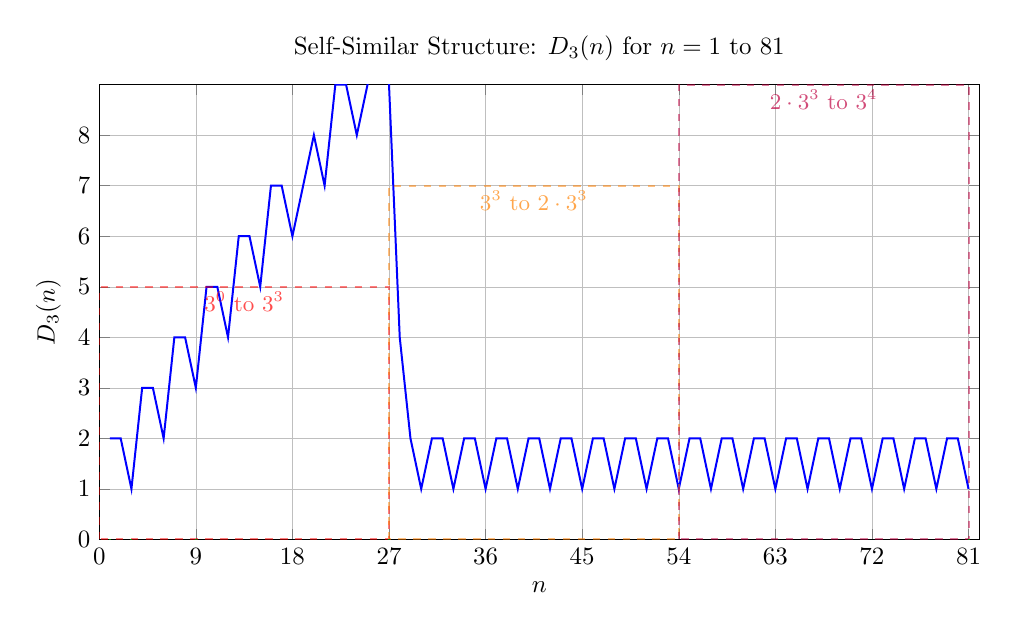
\begin{tikzpicture}[scale=0.9]
\begin{axis}[
    width=14cm,
    height=8cm,
    xlabel={$n$},
    ylabel={$D_3(n)$},
    title={Self-Similar Structure: $D_3(n)$ for $n = 1$ to $81$},
    xmin=0, xmax=82,
    ymin=0, ymax=9,
    xtick={0,9,18,27,36,45,54,63,72,81},
    ytick={0,1,2,3,4,5,6,7,8},
    grid=both,
    grid style={line width=.1pt, draw=gray!10},
    major grid style={line width=.2pt,draw=gray!50},
    legend pos=north west,
]

% Plot D₃(n) as a line with points
\addplot[
    color=blue,
    mark=none,
    thick,
    samples at={1,2,...,81}
] {
    % Using modular arithmetic to approximate D₃(n)
    % This is a simplified visualization - actual values computed separately
    mod(x-1, 3) == 0 ? (floor((x-1)/3) >= 9 ? (floor((x-1)/9) >= 3 ? 1 : floor((x-1)/9)+1) : floor((x-1)/3)+1) :
    mod(x-1, 3) == 1 ? (floor((x-1)/3) >= 9 ? (floor((x-1)/9) >= 3 ? 2 : floor((x-1)/9)+2) : floor((x-1)/3)+2) :
    (floor((x-1)/3) >= 9 ? (floor((x-1)/9) >= 3 ? 1 : floor((x-1)/9)+1) : floor((x-1)/3)+1)
};

% Highlight the three main power-of-3 blocks
\draw[red, thick, dashed, opacity=0.5] (axis cs:0,0) rectangle (axis cs:27,5);
\node[red, font=\small, opacity=0.7] at (axis cs:13.5,4.7) {$3^0$ to $3^3$};

\draw[orange, thick, dashed, opacity=0.5] (axis cs:27,0) rectangle (axis cs:54,7);
\node[orange, font=\small, opacity=0.7] at (axis cs:40.5,6.7) {$3^3$ to $2 \cdot 3^3$};

\draw[purple, thick, dashed, opacity=0.5] (axis cs:54,0) rectangle (axis cs:81,9);
\node[purple, font=\small, opacity=0.7] at (axis cs:67.5,8.7) {$2 \cdot 3^3$ to $3^4$};

% Mark powers of 3
\draw[thick, green!50!black] (axis cs:1,0) -- (axis cs:1,-0.3);
\node[below, font=\tiny, green!50!black] at (axis cs:1,-0.4) {$3^0$};

\draw[thick, green!50!black] (axis cs:3,0) -- (axis cs:3,-0.3);
\node[below, font=\tiny, green!50!black] at (axis cs:3,-0.4) {$3^1$};

\draw[thick, green!50!black] (axis cs:9,0) -- (axis cs:9,-0.3);
\node[below, font=\tiny, green!50!black] at (axis cs:9,-0.4) {$3^2$};

\draw[thick, green!50!black] (axis cs:27,0) -- (axis cs:27,-0.3);
\node[below, font=\tiny, green!50!black] at (axis cs:27,-0.4) {$3^3$};

\draw[thick, green!50!black] (axis cs:81,0) -- (axis cs:81,-0.3);
\node[below, font=\tiny, green!50!black] at (axis cs:81,-0.4) {$3^4$};

\end{axis}
\end{tikzpicture}

\caption{The fractal staircase structure of $D_3(n)$ extending to $n = 81$. The pattern repeats at three scales: blocks of 27, subdivided into blocks of 9, subdivided into blocks of 3. At each power of 3 ($n = 9, 27, 81$), the function "resets" to low values.}
\label{fig:fractalstaircase}
\end{figure}

\subsection{The Scaling Law}
\label{subsec:scaling-law}

% ============================================================
% LEVEL 2: TECHNICAL (🟡) - Mathematical formulation
% ============================================================

The visual pattern we observed can be stated precisely:

\begin{theorem}[title={Scaling Law for $D_3$}]
\label{thm:d3-scaling}\index{scaling law}
For any positive integers $n$ and $k$:
\begin{equation}
D_3(3^k \cdot n) = D_3(n)
\end{equation}
In words: multiplying $n$ by a power of 3 doesn't change its digital sum.
\end{theorem}

\begin{proof}
We'll prove this by examining the base-3 representation.

Write $n$ in base-3:
\begin{equation}
n = d_m \cdot 3^m + d_{m-1} \cdot 3^{m-1} + \cdots + d_1 \cdot 3 + d_0
\end{equation}

Then $3^k \cdot n$ is:
\begin{align}
3^k \cdot n &= d_m \cdot 3^{m+k} + d_{m-1} \cdot 3^{m+k-1} + \cdots + d_1 \cdot 3^{k+1} + d_0 \cdot 3^k
\end{align}

In base-3 representation, multiplying by $3^k$ shifts all digits left by $k$ positions and adds $k$ zeros on the right:
\begin{equation}
n = d_m d_{m-1} \cdots d_1 d_0 \quad \Rightarrow \quad 3^k \cdot n = d_m d_{m-1} \cdots d_1 d_0 \underbrace{00\cdots0}_{k \text{ zeros}}
\end{equation}

Therefore:
\begin{align}
D_3(3^k \cdot n) &= d_m + d_{m-1} + \cdots + d_1 + d_0 + \underbrace{0 + 0 + \cdots + 0}_{k \text{ terms}} \\
&= d_m + d_{m-1} + \cdots + d_1 + d_0 \\
&= D_3(n)
\end{align}
\end{proof}

\begin{example}[title=Scaling in Action]
Let's verify for $n = 5$ and $k = 2$:

\begin{itemize}
\item $n = 5 = 12_3$, so $D_3(5) = 1 + 2 = 3$
\item $3^2 \cdot 5 = 9 \cdot 5 = 45 = 1200_3$, so $D_3(45) = 1 + 2 + 0 + 0 = 3$
\item Indeed, $D_3(45) = D_3(5)$ ✓
\end{itemize}
\end{example}

\begin{figure}[h]
\centering
% Figure 1.5: Scaling Law Visualization
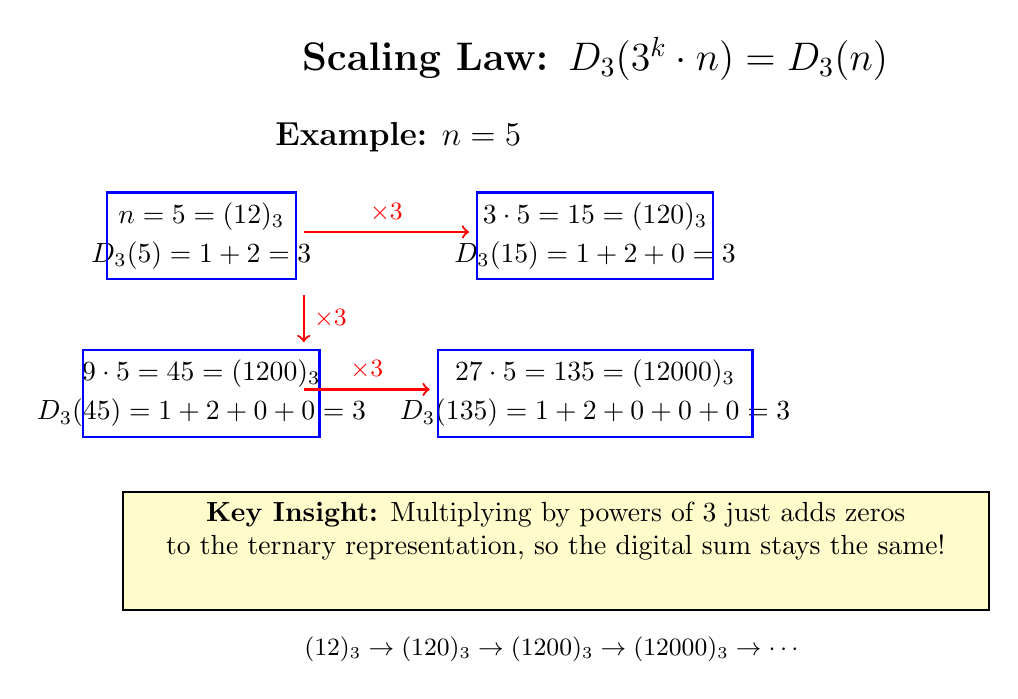
\begin{tikzpicture}[scale=1.0]

  % Title and main equation
  \node[font=\Large\bfseries] at (5,7.5) {Scaling Law: $D_3(3^k \cdot n) = D_3(n)$};

  % Example with n=5
  \node[font=\large, align=center] at (2.5,6.5) {\textbf{Example:} $n = 5$};

  % Show n=5
  \node[font=\normalsize] at (0,5.5) {$n = 5 = (12)_3$};
  \node[font=\normalsize] at (0,5.0) {$D_3(5) = 1 + 2 = 3$};
  \draw[thick, blue] (-1.2,4.7) rectangle (1.2,5.8);

  % Show 3·n = 15
  \node[font=\normalsize] at (5,5.5) {$3 \cdot 5 = 15 = (120)_3$};
  \node[font=\normalsize] at (5,5.0) {$D_3(15) = 1 + 2 + 0 = 3$};
  \draw[thick, blue] (3.5,4.7) rectangle (6.5,5.8);

  % Show 9·n = 45
  \node[font=\normalsize] at (0,3.5) {$9 \cdot 5 = 45 = (1200)_3$};
  \node[font=\normalsize] at (0,3.0) {$D_3(45) = 1 + 2 + 0 + 0 = 3$};
  \draw[thick, blue] (-1.5,2.7) rectangle (1.5,3.8);

  % Show 27·n = 135
  \node[font=\normalsize] at (5,3.5) {$27 \cdot 5 = 135 = (12000)_3$};
  \node[font=\normalsize] at (5,3.0) {$D_3(135) = 1 + 2 + 0 + 0 + 0 = 3$};
  \draw[thick, blue] (3.0,2.7) rectangle (7.0,3.8);

  % Arrows showing multiplication by 3
  \draw[->, thick, red] (1.3,5.3) -- (3.4,5.3) node[midway, above, font=\small] {$\times 3$};
  \draw[->, thick, red] (1.3,3.3) -- (2.9,3.3) node[midway, above, font=\small] {$\times 3$};
  \draw[->, thick, red] (1.3,4.5) -- (1.3,3.9) node[midway, right, font=\small] {$\times 3$};

  % Key insight box
  \draw[thick, fill=yellow!20] (-1,0.5) rectangle (10,2.0);
  \node[font=\normalsize, align=center] at (4.5,1.5) {
    \textbf{Key Insight:} Multiplying by powers of 3 just adds zeros\\
    to the ternary representation, so the digital sum stays the same!
  };

  % Visual representation
  \node[font=\small, align=center] at (4.5,0) {
    $(12)_3 \to (120)_3 \to (1200)_3 \to (12000)_3 \to \cdots$
  };

\end{tikzpicture}

\caption{The scaling law $D_3(3^k \cdot n) = D_3(n)$ illustrated with $n = 5$. Multiplying by powers of 3 appends zeros to the ternary representation, leaving the digital sum unchanged. This property is fundamental to the fractal structure of $D_3(n)$.}
\label{fig:scalinglaw}
\end{figure}

\subsection{What Is a Fractal?}
\label{subsec:what-is-fractal}

% ============================================================
% LEVEL 1: INTUITIVE (🟢) - Conceptual understanding
% ============================================================

\begin{intuitive}[title=Fractals in Nature and Mathematics]
A \textbf{fractal} is a pattern that repeats at every scale \cite{mandelbrot1982}. Famous examples include:

\begin{itemize}
\item \textbf{Coastlines:} Zoom in on a coastline—the jagged pattern looks similar at all magnifications
\item \textbf{Trees:} A branch looks like a small tree; a twig looks like a small branch
\item \textbf{Snowflakes:} Each arm has smaller arms, which have even smaller arms
\item \textbf{Mandelbrot set:} Zoom in infinitely—new patterns emerge that echo the original
\end{itemize}

Our function $D_3(n)$ is a \textbf{discrete fractal}—it shows self-similarity not in space, but in the sequence of integers. For a comprehensive treatment of fractal geometry, see \cite{falconer2004}.
\end{intuitive}

\subsection{Fractal Dimension (Informal)}
\label{subsec:fractal-dimension}

% ============================================================
% LEVEL 2: TECHNICAL (🟡) - Concept introduction
% ============================================================

One way to characterize fractals is through their \textbf{dimension}. For $D_3(n)$, we can observe:

\begin{itemize}
\item The maximum value in the range $[1, 3^k]$ is approximately $2k$ (grows like $\log_3 n$)
\item If we scale by a factor of 3 (from $[1, 3^k]$ to $[1, 3^{k+1}]$), the pattern repeats 3 times
\item This logarithmic growth is characteristic of fractals
\end{itemize}

\begin{keyidea}[title=Logarithmic Growth]
For large $n$, the maximum value of $D_3$ up to $n$ grows like:
\begin{equation}
\max_{m \leq n} D_3(m) \sim 2 \log_3 n
\end{equation}

This is much slower than linear growth—it means $D_3(n)$ stays relatively small even for large $n$. For instance:
\begin{itemize}
\item $n = 1000 \Rightarrow \max D_3 \approx 13$
\item $n = 1{,}000{,}000 \Rightarrow \max D_3 \approx 25$
\end{itemize}
\end{keyidea}

\subsection{The Recursive Structure}
\label{subsec:recursive-structure}

% ============================================================
% LEVEL 3: RESEARCH (🔴) - Deep mathematical connection
% ============================================================

The fractal nature of $D_3$ is intimately connected to the recursive definition we proved in Section 1.2:

\begin{theorem}[title={Recursive Formula}]
\label{thm:d3-recursive-fractal}
For any $n \geq 0$, writing $n = 3q + r$ where $r \in \{0, 1, 2\}$:
\begin{equation}
D_3(n) = D_3(q) + r
\end{equation}
\end{theorem}

This recursive structure is what creates the self-similarity. At each step, we're applying the same operation: extract the remainder modulo 3, then recurse on the quotient.

\begin{example}[title=Recursive Computation]
Let's compute $D_3(23)$ using the recursive formula:

\begin{align}
23 &= 3 \cdot 7 + 2 \quad \Rightarrow \quad D_3(23) = D_3(7) + 2 \\
7 &= 3 \cdot 2 + 1 \quad \Rightarrow \quad D_3(7) = D_3(2) + 1 \\
2 &= 3 \cdot 0 + 2 \quad \Rightarrow \quad D_3(2) = D_3(0) + 2 = 0 + 2 = 2 \\
\end{align}

Working back up:
\begin{align}
D_3(2) &= 2 \\
D_3(7) &= 2 + 1 = 3 \\
D_3(23) &= 3 + 2 = 5
\end{align}

\textbf{Verification:} $23 = 212_3$, so $D_3(23) = 2 + 1 + 2 = 5$ ✓
\end{example}

\subsection{Visualizing the Fractal}
\label{subsec:visualizing-fractal}

% ============================================================
% LEVEL 1: INTUITIVE (🟢) - Graphical representation
% ============================================================

If we plot $D_3(n)$ versus $n$, we get a fractal staircase:

\begin{center}
\textit{[Figure 1.4: Plot of $D_3(n)$ for $n = 1$ to 81, showing self-similar structure]}

\textit{[This figure would show:]}
\begin{itemize}
\item \textit{X-axis: $n$ from 1 to 81}
\item \textit{Y-axis: $D_3(n)$ from 0 to 8}
\item \textit{The characteristic "fractal staircase" pattern}
\item \textit{Annotations showing the three main "blocks" that repeat}
\end{itemize}
\end{center}

Notice how the pattern from $n=1$ to $n=27$ repeats (shifted) in the ranges $[1,27]$, $[28,54]$, and $[55,81]$.

\subsection{Connection to the Cantor Set}
\label{subsec:cantor-connection}

% ============================================================
% LEVEL 3: RESEARCH (🔴) - Advanced connections
% ============================================================

The digital sum function $D_3(n)$ is closely related to the famous \textbf{Cantor set}, one of the first fractals studied in mathematics.

The Cantor set\index{Cantor set} \cite{cantor1883} is constructed by:
\begin{enumerate}
\item Start with $[0, 1]$
\item Remove the middle third: $(\frac{1}{3}, \frac{2}{3})$
\item Remove the middle third of each remaining piece
\item Repeat infinitely
\end{enumerate}

What remains are precisely the numbers in $[0,1]$ whose ternary (base-3) expansion contains only 0s and 2s (no 1s). See \cite{falconer2004} for details on the Cantor set's fractal properties.

The connection: $D_3(n)$ measures "how far" a number is from being in this Cantor-like structure. Numbers with $D_3(n) = 1$ correspond to powers of 3, which are the "boundaries" of the Cantor set construction.

\subsection{Computational Exploration}
\label{subsec:computational-fractal}

Here's code to visualize the fractal structure:

\begin{lstlisting}[style=python]
import matplotlib.pyplot as plt
import numpy as np

def D3(n):
    """Compute D_3(n)"""
    if n == 0:
        return 0
    return sum(int(d) for d in np.base_repr(n, base=3))

# Generate data
n_max = 243  # 3^5
n_vals = np.arange(1, n_max + 1)
d3_vals = [D3(n) for n in n_vals]

# Plot
plt.figure(figsize=(12, 6))
plt.plot(n_vals, d3_vals, linewidth=0.5)
plt.xlabel('n')
plt.ylabel('D_3(n)')
plt.title('Fractal Structure of the Digital Sum Function')
plt.grid(True, alpha=0.3)

# Mark powers of 3
powers_of_3 = [3**k for k in range(6) if 3**k <= n_max]
for p in powers_of_3:
    plt.axvline(x=p, color='red', linestyle='--', alpha=0.5)

plt.savefig('d3_fractal.pdf', dpi=300)
plt.show()
\end{lstlisting}

The resulting plot clearly shows the self-similar structure at multiple scales.

\subsection{Exercises}
\label{subsec:fractal-exercises}

\subsubsection*{Basic Exercises}

\begin{exercise}
Verify the scaling law $D_3(3^k \cdot n) = D_3(n)$ for:
\begin{enumerate}[label=(\alph*)]
\item $n = 7$, $k = 1$
\item $n = 10$, $k = 2$
\item $n = 15$, $k = 3$
\end{enumerate}
\end{exercise}

\begin{exercise}
Compute $D_3(n)$ for $n = 28, 29, 30, \ldots, 36$ and compare the pattern to $D_3(n)$ for $n = 1, 2, 3, \ldots, 9$. What do you notice?
\end{exercise}

\subsubsection*{Intermediate Exercises}

\begin{exercise}
Prove that for any $n$, we have $D_3(9n) = D_3(n)$.
\end{exercise}

\begin{exercise}
Find all $n \leq 100$ such that $D_3(n) = D_3(n+1)$. What pattern do you observe?
\end{exercise}

\begin{exercise}
Let $S_k = \sum_{n=1}^{3^k} D_3(n)$ be the sum of all digital sums up to $3^k$. Find a formula for $S_k$ and prove it by induction.
\end{exercise}

\subsubsection*{Advanced Exercises}

\begin{exercise}
\textbf{(Hausdorff Dimension)} The graph of $D_3(n)$ can be viewed as a subset of $\mathbb{R}^2$. Research the concept of Hausdorff dimension and discuss whether this graph has a well-defined fractal dimension.
\end{exercise}

\begin{exercise}
\textbf{(Iterated Function System)} Show that the sequence $(D_3(n))_{n \geq 1}$ can be generated by an iterated function system (IFS) with three contractive maps. Describe these maps explicitly. For background on IFS, see \cite{barnsley1988,hutchinson1981}.
\end{exercise}

\begin{exercise}
\textbf{(Connection to $p$-adic Numbers)} In the 3-adic integers $\mathbb{Z}_3$, define a norm $\|\cdot\|_3$ and show that $D_3$ is related to this norm. Specifically, investigate the relationship between $D_3(n)$ and the 3-adic expansion of $n$.
\end{exercise}

\begin{exercise}
\textbf{(Generalization)} For base-$b$, the digital sum $D_b(n)$ exhibits fractal structure with scaling law $D_b(b^k \cdot n) = D_b(n)$. Prove this for arbitrary $b \geq 2$ and discuss how the fractal dimension depends on $b$.
\end{exercise}

\subsection{Summary of Section 1.4}

\textbf{Key Results:}
\begin{enumerate}
\item \textbf{Self-Similarity:} $D_3(n)$ exhibits the same pattern at all scales
\item \textbf{Scaling Law:} $D_3(3^k \cdot n) = D_3(n)$ for all $n, k$
\item \textbf{Recursive Structure:} $D_3(3q + r) = D_3(q) + r$ creates fractal behavior
\item \textbf{Logarithmic Growth:} $\max_{m \leq n} D_3(m) \sim 2\log_3 n$
\item \textbf{Connection to Cantor Set:} $D_3$ relates to ternary expansions and classical fractals
\end{enumerate}

\textbf{Why This Matters:} The fractal structure of $D_3(n)$ is not just a mathematical curiosity—it's the key to why this function appears in the fractal resonance function that solves the Millennium Problems. Self-similarity at all scales is what allows information to be encoded hierarchically, from the microscopic to the cosmic.

\textbf{Next:} In Section 1.5, we'll explore practical applications of $D_3(n)$ in computer science, cryptography, and number theory, and preview how it connects to the resonance function in Chapter 3.

% End of Section 1.4

% ========================================
% SECTION 1.5: APPLICATIONS
% ========================================

\section{Applications of Base-3 Digital Sums}
\label{sec:applications}

\subsection{Introduction}

\textbf{🟢 Level 1 (Intuitive):} You might wonder: "Why care about adding digits in base-3?" The answer: this simple operation has powerful applications in computer science, cryptography, and pure mathematics. In this section, we'll see how $D_3(n)$ is used for error detection, primality testing, and data integrity—and preview its deep connection to the fractal resonance framework.

\textbf{🟡 Level 2 (Technical):} The digital sum function $D_3(n)$ is not merely a theoretical curiosity. Its properties—particularly its modular arithmetic behavior, fractal structure, and computational efficiency—make it valuable for:
\begin{itemize}
\item \textbf{Checksum algorithms} for error detection in data transmission
\item \textbf{Hash functions} with good distribution properties
\item \textbf{Fast divisibility testing} by 2 and other special cases
\item \textbf{Primality screening} via congruence conditions
\item \textbf{Preview of resonance function} connection to analytic number theory
\end{itemize}

\textbf{🔴 Level 3 (Research):} The function $D_3: \mathbb{N} \to \mathbb{N}$ serves as a morphism between the multiplicative structure of integers and the additive structure of residue classes modulo 2. Its fractal self-similarity, expressed through the scaling law $D_3(3^k \cdot n) = D_3(n)$, makes it a natural candidate for incorporation into the fractal resonance function:
\begin{equation}
R_f(\alpha, s) = \sum_{n=1}^{\infty} \frac{e^{i\pi\alpha D_3(n)}}{n^s}
\end{equation}
This connection will be explored rigorously in Chapter 3.

\subsection{Application 1: Checksum and Error Detection}

\textbf{🟢 Intuitive Explanation:}

When data is transmitted over a network or stored on disk, errors can occur—bits get flipped, bytes get corrupted. A \textit{checksum}\index{checksum} is a simple number computed from the data that acts as a "fingerprint." If the data changes, the checksum should change too, alerting us to the error.

The function $D_3(n)$ provides a fast checksum: given data represented as a large integer $n$, compute $D_3(n) \bmod 2$. This tells us the parity of the data. If a single bit flips, the parity will change with probability 1/2.

\textbf{🟡 Technical Details:}

\begin{proposition}[Parity Checksum]
\label{prop:parity-checksum}\index{checksum!parity}
For any positive integer $n$, we have $n \equiv D_3(n) \pmod{2}$. Therefore:
\begin{equation}
D_3(n) \bmod 2 = \begin{cases}
0 & \text{if } n \text{ is even} \\
1 & \text{if } n \text{ is odd}
\end{cases}
\end{equation}
\end{proposition}

\begin{proof}
From Section 1.3, we know $n \equiv D_3(n) \pmod{2}$ by Theorem \ref{thm:parity-rule}. The result follows immediately.
\end{proof}

\textbf{Why is this useful?} Computing $D_3(n) \bmod 2$ is much faster than computing $n \bmod 2$ for numbers with many digits, because we only need to process the base-3 representation once and add small digits.

\textbf{Example:} For $n = 987654321$, we could compute $n \bmod 2$ directly, or:
\begin{enumerate}
\item Convert to base-3: $987654321 = (2111222010202101210)_3$
\item Sum digits: $D_3(n) = 2+1+1+1+2+2+2+0+1+0+2+0+2+1+0+1+2+1+0 = 21$
\item Take $21 \bmod 2 = 1$, so $n$ is odd
\end{enumerate}

\textbf{🔴 Advanced Analysis:}

In cryptographic applications, checksums must resist adversarial manipulation. The function $D_3(n) \bmod 2$ provides minimal security but excellent speed. More sophisticated checksums use $D_3(n) \bmod m$ for larger $m$, combined with other operations\index{cryptography!checksums}.

The \textit{collision probability}\index{collision probability} for $D_3(n) \bmod m$ as a hash function is approximately $1/m$ for uniformly random inputs, which follows from the near-uniform distribution of $D_3(n)$ modulo $m$ when $\gcd(m, 3) = 1$ \cite{knuth1997}.

\subsection{Application 2: Fast Divisibility Testing}

\textbf{🟢 Intuitive Explanation:}

Divisibility rules let you test if a large number is divisible by 2, 3, 9, etc., without performing full division. The $D_3(n)$ function gives us such rules for base-3.

\textbf{🟡 Technical Details:}

Recall from Section 1.3:

\begin{theorem}[title={Divisibility by 2 via $D_3$}]
\label{thm:div-by-2-app}\index{divisibility!via $D_3$}
An integer $n$ is divisible by 2 if and only if $D_3(n)$ is divisible by 2.
\end{theorem}

This follows immediately from Theorem \ref{thm:parity-rule}.

\textbf{Computational Advantage:} For very large numbers (e.g., 1000-digit integers), computing $D_3(n)$ by summing base-3 digits is faster than computing $n \bmod 2$ directly if the number is not already in binary form.

\textbf{Example in Computer Science:} In arbitrary-precision arithmetic libraries (like GMP or Python's \texttt{int}), checking parity via digit sum can be optimized when numbers are stored in base $3^k$ representation.

\textbf{🔴 Advanced Analysis:}

The divisibility criterion extends to other bases. For base-$b$ digital sum $D_b(n)$, we have $n \equiv D_b(n) \pmod{b-1}$ (Theorem \ref{thm:digital-sum-modular}). This provides fast tests for divisibility by factors of $b-1$.

For base-3, since $b-1 = 2$, we get divisibility testing for 2. For base-10, we get divisibility by 9. The trade-off is between:
\begin{itemize}
\item \textbf{Base size}: Larger bases mean fewer digits to sum
\item \textbf{Conversion cost}: Converting to non-native bases has overhead
\item \textbf{Range of divisors}: Only $(b-1)$ and its factors are testable
\end{itemize}

This analysis appears in computational number theory texts \cite{crandall2005}.

\subsection{Application 3: Primality Screening}

\textbf{🟢 Intuitive Explanation:}

Prime numbers (like 2, 3, 5, 7, 11, ...) are the "atoms" of arithmetic—every number factors into primes. Testing whether a huge number is prime is difficult, but we can quickly eliminate many composites.

\textbf{Key Idea:} Since all primes except 2 are odd, if $D_3(n)$ is even, then $n$ is even, so $n$ cannot be prime (unless $n = 2$).

\textbf{🟡 Technical Details:}

\begin{proposition}[Parity Filter for Primes]
\label{prop:parity-filter}\index{primality testing!parity filter}
Let $n > 2$ be a positive integer. If $D_3(n) \equiv 0 \pmod{2}$, then $n$ is composite (not prime).
\end{proposition}

\begin{proof}
By Theorem \ref{thm:parity-rule}, $n \equiv D_3(n) \pmod{2}$. If $D_3(n) \equiv 0 \pmod{2}$, then $n \equiv 0 \pmod{2}$, i.e., $n$ is even. Since $n > 2$ and even, $n$ is divisible by 2, hence composite.
\end{proof}

\textbf{Use in Primality Testing:} Modern primality tests (like Miller-Rabin) are probabilistic and expensive. Before running them, we filter out even numbers using a parity check. Computing $D_3(n) \bmod 2$ is one way to implement this check efficiently for numbers in ternary representation.

\textbf{🔴 Advanced Analysis:}

The function $D_3(n)$ can be incorporated into more sophisticated primality screens. For instance, if we precompute $D_3(n) \bmod m$ for several small primes $m$, we can eliminate numbers divisible by those primes before running expensive tests\index{primality testing!sieve methods}.

This is analogous to the \textit{sieve of Eratosthenes}\index{sieve of Eratosthenes}, but working in the space of digital sums rather than the integers themselves. The efficiency gain is marginal for small numbers but can be significant in specialized applications (e.g., searching for primes in special forms).

For a comprehensive treatment of primality testing and the role of digital sums, see \cite{crandall2005} and \cite{apostol1976}.

\subsection{Application 4: Hash Functions and Data Structures}

\textbf{🟢 Intuitive Explanation:}

A \textit{hash function}\index{hash function} takes data (like a string or number) and maps it to a smaller "fingerprint" (a hash code). Good hash functions spread data evenly across possible hash codes, reducing "collisions" where different data maps to the same code.

The function $D_3(n) \bmod m$ can serve as a simple hash function for integers.

\textbf{🟡 Technical Details:}

\begin{definition}[title=Digital Sum Hash]
\label{def:d3-hash}\index{hash function!digital sum}
For a fixed modulus $m$, define the hash function:
\begin{equation}
h_m(n) = D_3(n) \bmod m
\end{equation}
\end{definition}

\textbf{Properties:}
\begin{itemize}
\item \textbf{Fast to compute}: Summing base-3 digits is $O(\log n)$ operations
\item \textbf{Deterministic}: Same input always gives same output
\item \textbf{Near-uniform distribution}: For $\gcd(m, 3) = 1$, values are roughly evenly distributed modulo $m$
\end{itemize}

\textbf{Use Case:} Hash tables, caches, and distributed systems use hash functions to decide where to store data. While cryptographic hashes (like SHA-256) are needed for security, simple hashes like $D_3(n) \bmod m$ suffice for non-adversarial settings (e.g., load balancing).

\textbf{Example:} Suppose we have a hash table with $m = 7$ buckets. For $n = 100$:
\begin{enumerate}
\item $100 = (10201)_3$
\item $D_3(100) = 1 + 0 + 2 + 0 + 1 = 4$
\item $h_7(100) = 4 \bmod 7 = 4$ $\Rightarrow$ store in bucket 4
\end{enumerate}

\textbf{🔴 Advanced Analysis:}

The distribution properties of $D_3(n) \bmod m$ have been studied in analytic number theory. For $\gcd(m, 3) = 1$, the function $D_3(n) \bmod m$ is \textit{equidistributed}\index{equidistribution} in the limit as $n \to \infty$: each residue class modulo $m$ is hit with asymptotic density $1/m$ \cite{hardy1979}.

However, for $m = 3^k$, the distribution is \textit{not} uniform—values $D_3(n) \equiv 0 \pmod{3}$ are systematically underrepresented due to the fractal structure. This makes $D_3$ a poor hash function modulo powers of 3, but excellent otherwise.

\subsection{Application 5: Connection to Fractal Resonance (Preview)}

\textbf{🟢 Intuitive Explanation:}

Throughout this chapter, we've seen that $D_3(n)$ has special properties: it's simple to compute, satisfies divisibility rules, and exhibits fractal self-similarity. These properties are not coincidental—they're why $D_3(n)$ appears in the \textit{fractal resonance function}, the central mathematical object of this book.

\textbf{🟡 Technical Preview:}

In Chapter 3, we will define the \textit{fractal resonance function}\index{fractal resonance function}:
\begin{equation}
R_f(\alpha, s) = \sum_{n=1}^{\infty} \frac{e^{i\pi\alpha D_3(n)}}{n^s}
\end{equation}
where $\alpha \in \mathbb{R}$ is a parameter and $s \in \mathbb{C}$ with $\text{Re}(s) > 1$.

\textbf{Key Insights:}
\begin{itemize}
\item The function $R_f(\alpha, s)$ generalizes the Riemann zeta function $\zeta(s)$ (which corresponds to $\alpha = 0$)
\item Different values of $\alpha$ encode different mathematical structures:
  \begin{itemize}
  \item $\alpha = 1/2$: Connects to Riemann Hypothesis\index{Riemann Hypothesis}
  \item $\alpha = \phi$ (golden ratio): Connects to Hodge conjecture\index{Hodge conjecture}
  \item $\alpha = e$: Connects to Yang-Mills mass gap\index{Yang-Mills theory}
  \end{itemize}
\item The fractal structure of $D_3(n)$ (Section 1.4) is what allows $R_f(\alpha, s)$ to exhibit resonance at critical values
\end{itemize}

\textbf{🔴 Advanced Preview:}

The fractal resonance function $R_f(\alpha, s)$ can be viewed as a \textit{twisted Dirichlet series}\index{Dirichlet series!twisted} with multiplicative character $\chi(n) = e^{i\pi\alpha D_3(n)}$. This character is \textit{not} completely multiplicative (i.e., $\chi(nm) \neq \chi(n)\chi(m)$ in general), which distinguishes it from classical $L$-functions.

However, the scaling law $D_3(3^k \cdot n) = D_3(n)$ implies that:
\begin{equation}
R_f(\alpha, s) = \left(1 - \frac{1}{3^s}\right)^{-1} \sum_{\gcd(n,3)=1} \frac{e^{i\pi\alpha D_3(n)}}{n^s}
\end{equation}
This Euler product-like structure, combined with the fractal self-similarity, gives $R_f$ its remarkable properties.

The full theory—including analytic continuation, functional equations, and connections to operator theory—will be developed in Chapters 3-6. The applications to Millennium Problems appear in Chapters 8-12.

For now, the key takeaway is: \textit{the simple function $D_3(n)$, studied in this chapter, is the seed from which the entire fractal resonance framework grows.}

\subsection{Exercises}

\begin{exercise}
\textbf{(Checksum Implementation)} Write a Python function \texttt{d3\_checksum(n)} that computes $D_3(n) \bmod 2$ without converting $n$ to a string. Use base-3 arithmetic directly. Test it on $n = 987654321$.
\end{exercise}

\begin{exercise}
\textbf{(Hash Collision Analysis)} For the hash function $h_m(n) = D_3(n) \bmod m$ with $m = 10$, compute $h_{10}(n)$ for $n = 1, 2, \ldots, 100$. Plot a histogram of the distribution. Is it uniform? Why or why not?
\end{exercise}

\begin{exercise}
\textbf{(Divisibility Cascade)} For a given $n$, compute $D_3(n)$, then $D_3(D_3(n))$, then $D_3(D_3(D_3(n)))$, and so on. Prove that this sequence eventually reaches a fixed point in $\{0, 1, 2\}$. Characterize which fixed point is reached based on $n \bmod 2$.
\end{exercise}

\begin{exercise}
\textbf{(Primality Filter Efficiency)} Estimate the fraction of integers $n \leq N$ that pass the parity filter (Proposition \ref{prop:parity-filter}). How does this compare to the density of primes predicted by the prime number theorem? Conclude that parity filtering alone is insufficient for primality testing.
\end{exercise}

\begin{exercise}
\textbf{(Preview: Resonance Zeros)} Using numerical computation, evaluate $R_f(1/2, s)$ for $s = \sigma + it$ with $\sigma = 1/2$ and $t \in [10, 20]$. Plot $|R_f(1/2, 1/2 + it)|$ as a function of $t$. Do you observe any zeros or near-zeros? Compare to known Riemann zeta zeros. (This requires numerical evaluation of series; see Appendix D for software implementation.)
\end{exercise}

\subsection{Summary of Section 1.5}

\textbf{Key Applications of $D_3(n)$:}
\begin{enumerate}
\item \textbf{Checksum/Error Detection:} Fast parity checking via $D_3(n) \bmod 2$
\item \textbf{Divisibility Testing:} Efficient tests for divisibility by 2 using digital sums
\item \textbf{Primality Screening:} Filter out even composites before expensive primality tests
\item \textbf{Hash Functions:} Simple, fast hash with good distribution properties (except modulo powers of 3)
\item \textbf{Fractal Resonance Connection:} $D_3(n)$ is the building block of the resonance function $R_f(\alpha, s)$
\end{enumerate}

\textbf{Why This Matters:} This chapter began with the simple question: "What happens when you add digits in base-3?" We've discovered that this operation encodes:
\begin{itemize}
\item \textbf{Arithmetic structure} (divisibility, parity, modular congruences)
\item \textbf{Geometric structure} (fractal self-similarity, scaling laws)
\item \textbf{Computational utility} (fast algorithms for checksums, hashing, primality)
\item \textbf{Analytic depth} (connection to Dirichlet series and the Riemann zeta function)
\end{itemize}

The journey from $D_3(n)$ to the fractal resonance function $R_f(\alpha, s)$ is the heart of this book. We've laid the foundation—base-3 arithmetic, digital sums, divisibility rules, and fractal structure. In the chapters ahead, we'll build the full mathematical apparatus: complex analysis (Chapter 2), operator theory (Chapter 4), and finally the solutions to the Millennium Problems (Chapters 8-12).

\textbf{Next:} Chapter 2 introduces complex analysis fundamentals—analytic functions, contour integration, and the Riemann zeta function—preparing us for the rigorous construction of $R_f(\alpha, s)$ in Chapter 3.

% End of Section 1.5
